\section{Trave a doppia rastremazione}
\begin{pycode}[TraveDoppiaRastremazione]
beamType = 'DoppiaRastremazione'
# beamType = 'Curva'
# beamType = 'Centinata'

timberType = 'lamellare'
# timberType = 'massiccio'

glulam_class = 'GL28h'
# N/mm2
f_mk = 28
f_vk = 3.5
f_c90k = 2.5
f_t90k = 0.5
E0mean = 12600
E005 = 10500
Gmean = 650
G05 = 540.0

gammaM = 1.45
kmod = 0.9

alpha = 3.5 # in gradi °
b = 240
h_ap = 1800-500 # altezza apice
h_0 = 1315-500 # altezza appoggio
l = 16000 

alpha = np.radians(alpha)

# volume della trave 
V_b = (h_ap + h_0) * l/2 * b 
V_b = V_b/10**9 # da mm3 a m3

# vale solo per la trave a doppia rastremazione:
# volume della zona di colmo
# formula alternativa: b * h_ap**2 * (1 - 0.25 * np.tan(alpha)) / 10**9
h_ap_05 = h_ap - np.tan(alpha)*0.5*h_ap
V_colmo =  (h_ap_05 + h_ap) * 0.5*h_ap * b
V_colmo = V_colmo/10**9

# volume zona di colmo per la normativa
V = min(2/3 * V_b , V_colmo)

V_0 = 0.01

# Sollecitazioni di progetto:
Q = 19.56 #kN/m == N/mm

M_d = Q * l**2 / 8
V_d = Q *l / 2

### Inizio della verifica:

## Parte di trave a doppia rastremazione

# Flessione
f_md = kmod * f_mk / gammaM

t = 30 # spessore lamelle LVL
r_in = 17000 #raggio interno se curva o centinata. altrimenti non serve
if beamType == 'DoppiaRastremazione':
    k_r = 1
else:
    k_r = 1 if r_in/t >240 else 0.76 + 0.001 * r_in/t

alpha_ap = np.radians(3.5) # vedi la figura
if beamType == 'DoppiaRastremazione':
    k_l = k_1 = 1 + 1.4*np.tan(alpha_ap) + 5.4*np.tan(alpha_ap)**2
else:
    k_1 = 1 + 1.4*np.tan(alpha_ap) + 5.4*np.tan(alpha_ap)**2
    k_2 = 0.35 - 8*np.tan(alpha_ap)
    k_3 = 0.6 + 8.3*np.tan(alpha_ap) - 7.8*np.tan(alpha_ap)**2
    k_4 = 6*np.tan(alpha_ap)**2
    r = r_in + 0.5 * h_ap
    k_l = k_1 + k_2*(h_ap/r) + k_3*(h_ap/r)**2 + k_4*(h_ap/r)**3
sigma_md = k_l * 6 * M_d / (b*h_ap**2) # nel punto in mezzeria

#######
# Trazione 90 all'apice
k_dis =  1.4 if beamType == 'DoppiaRastremazione' or  beamType == 'Curva' else  1.7
k_vol = 1 if timberType == 'massiccio' else (V_0/V)**0.2 

f_t90d = f_t90k * kmod / gammaM
k_dis * k_vol * f_t90d

# k_p solo per trave doppia rastremazione. aggiungere le altre!
k_p = 0.2 * np.tan(alpha) 

def sigma_t90d(M,b,h,k_p):
    sigma_t90d = 6 * M / (b*h**2) * k_p
    return sigma_t90d

sigma_t90d_ap = sigma_t90d(M_d,b,h_ap,k_p)

###
# Taglio + trazione a 0.5 ap
x_05ap = l/2 - 0.5*h_ap
V_05ap = Q * (2 * 0.5*h_ap) / 2
M_05ap = V_d * (l/2 - 0.5*h_ap) - Q*(l/2 - 0.5*h_ap)**2 / 2

f_vd = f_vk * kmod / gammaM

b_eff = 2.5/f_vk * b
tau_d_05ap = 1.5*V_05ap/(b_eff*h_ap_05)
sigma_t90d_05ap = sigma_t90d(M_05ap , b , h_ap_05 , k_p)

####
## Zona a rastremazione semplice
x_max = l * h_0 / (2*h_ap)
h_max = h_ap - np.tan(alpha)*(l/2 - x_max) # altezza corrispondente alla x_max
M_xmax = V_d * x_max - Q*x_max**2 / 2
sigma_md_max = 6*M_xmax / (b*h_max**2)

f_c90d = f_c90k * kmod / gammaM

k_mAlpha_compressione = 1 / np.sqrt(1 + (np.tan(alpha)*f_md/(1.5*f_vd))**2 + ((np.tan(alpha))**2*f_md/f_c90d)**2 )

k_def = 0.6
\end{pycode}

\begin{pysub}[TraveDoppiaRastremazione]
\begin{figure}[H]
    \centering
    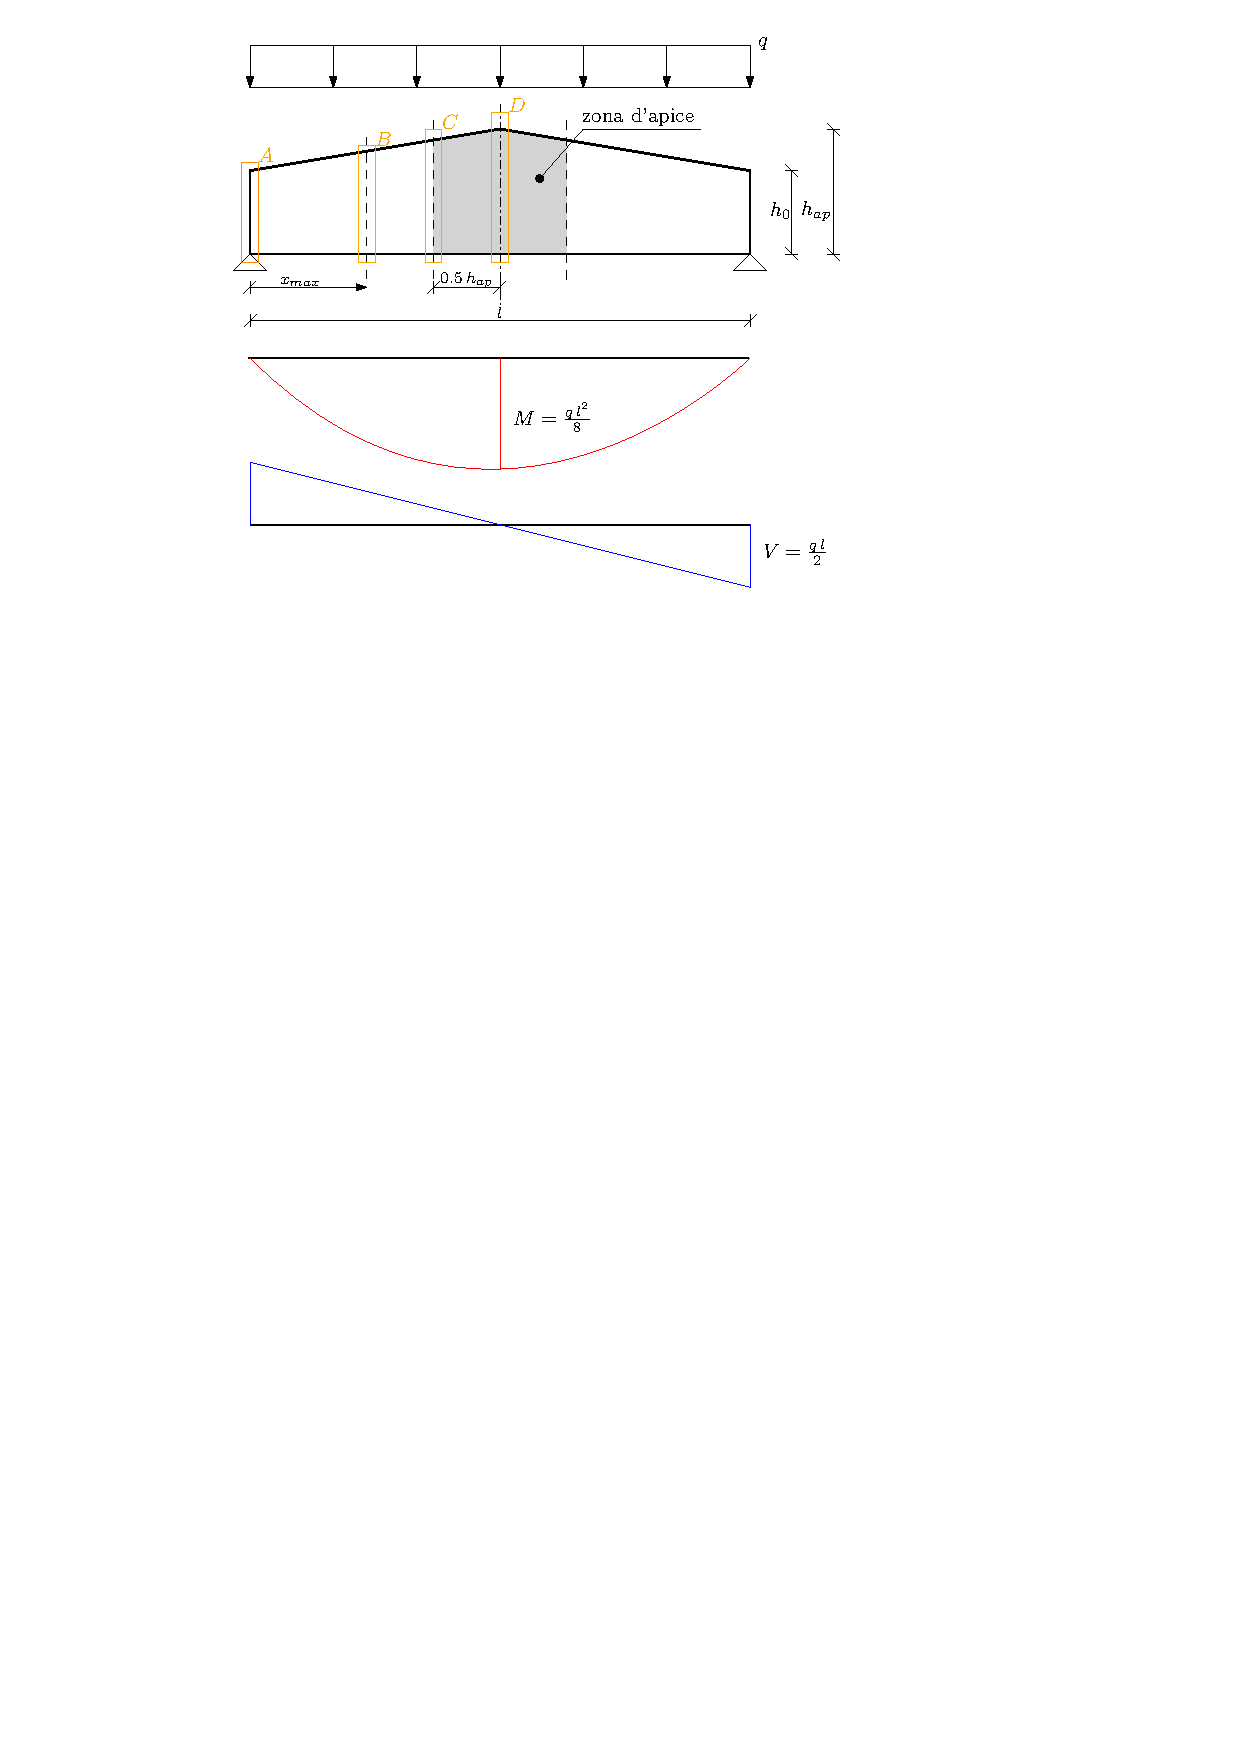
\includegraphics[]{IMG/TraveDoppiaRastremazione.pdf}
    \caption{Indicazione della nomenclatura adottata per le zone di verifica lungo lo sviluppo della trave e delle condizioni di carico assunte}
    \label{fig:TraveDoppiaRastremazione}
\end{figure}

\begin{table}[H]
    \centering
    \caption{Azioni di progetto nei punti di sezione indicati in figura per la trave a doppia rastremazione}
    \begin{tabular}{c  S[table-format=4.1] S[table-format=4.3] S[table-format=3.3]}
        \toprule
		%\multicolumn{4}{c}{Azioni di progetto nei punti di sezione}\\
        Sezione & \multicolumn{1}{c}{$x$ [\si{\milli\metre}]} & \multicolumn{1}{c}{$M_d$ [\si{\kilo\newton\metre}]}& \multicolumn{1}{c}{$V_d$ [\si{\kilo\newton}]} \\
        \midrule
        A & 0. 0               & 0.0                      & !{round(V_d/10**3,3)}   \\
        B & !{round(x_max,1)}  & !{round(M_xmax/10**6,3)} &                        \\
        C & !{round(x_05ap,1)} & !{round(M_05ap/10**6,3)} & !{round(V_05ap/10**3,3)}\\
        D & !{round(l/2,1)}    & !{round(M_d/10**6,3)}    & 0.0						\\
        \bottomrule
    \end{tabular}
\end{table} 
\begin{table}[H]
    \centering
    \caption{Valori di progetto per la verifica della trave a doppia rastremazione}
    \begin{tabular}{lS[table-format=2.1] @{\hspace{2cm}} lS[table-format=2.3]@{\hspace{2cm}} lS[table-format=5.1]}
        \toprule
		\multicolumn{6}{c}{Valori geometrici e coefficienti di esposizione o durata del carico}\\
        \midrule
		$b$      & \SI{!{b}}{\milli\metre}     & $h_{ap}$        & \SI{!{h_ap}}{\milli\metre}   & $\alpha$ & \SI{!{round(np.rad2deg(alpha),1)}}{\degree} \\ 
		$h_0$    & \SI{!{h_0}}{\milli\metre}                    & $l$           & \SI{!{l}}{\milli\metre}   & $\alpha_{ap}$ & \SI{!{round(np.rad2deg(alpha_ap),1)}}{\degree} \\
        $\gamma_M$      & \SI{!{gammaM}}{}     & $k_{mod}$        & \SI{!{kmod}}{}   & $k_{def}$ & \SI{!{k_def}}{} \\
        \midrule
        \multicolumn{6}{c}{Valori di resistenza GL28h [\si{\mega\pascal}] } \\
        \midrule
        $f_{m,k}$    & !{f_mk}   & $f_{m,d}$    & !{round(f_md,3)}  & $E_{0,mean}$ & !{E0mean} \\
        $f_{v,k}$    & !{f_vk}   & $f_{v,d}$    & !{round(f_vd,3)}  & $E_{0,05}$   & !{E005} \\
        $f_{c,90,k}$ & !{f_c90k} & $f_{c,90,d}$ & !{round(f_c90d,3)} & $G_{mean}$   & !{Gmean} \\
        $f_{t,90,k}$ & !{f_t90k} & $f_{t,90,d}$ & !{round(f_t90d,3)} &  $G_{05}$     & !{G05}\\
        \bottomrule
    \end{tabular}
\end{table} 


In riferimento alla nomenclatura delle sezioni mostrata in figura \ref{fig:TraveDoppiaRastremazione} si riportano ora le verifiche svolte.
\subsection{Flessione -- Sezione D}
\begin{equation} 
    \sigma_{m,d} \leq k_r \cdot f_{m,d} 
\end{equation}
Avendo la trave a doppia rastremazione un raggio $r_{in} = \infty$ si ha  
\begin{equation}
    k_{r} =
    \begin{cases}
        1 & \text{se \quad $\dfrac{r_{in}}{t} \geq 240$} \\
        0.76 + 0.001 \dfrac{r_{in}}{t} & \text{se \quad $\dfrac{r_{in}}{t} < 240$}
    \end{cases}
    \quad =  !{round(k_r,3)} \quad .
\end{equation} 
La sollecitazione in mezzeria vale
\begin{equation}
\sigma_{m,d} = k_l \frac{6 \cdot M_{ap,d}}{b \cdot h_{ap}^2} = !{round(k_l,3)} 
\frac{  6 \cdot \SI{!{round(M_d/10**6,3)}e6}{\newton\milli\metre}  }{\SI{!{b}} {\milli\metre} \cdot (\SI{!{h_ap}} {\milli\metre})^2} = \SI{!{round(sigma_md,3)}}{\mega\pascal}
\end{equation}
dove 
\begin{equation}
    k_l = k_1 + k_2 \left( \dfrac{h_{ap}}{r} \right) + k_3 \left( \dfrac{h_{ap}}{r} \right)^2 + k_4 \left( \dfrac{h_{ap}}{r} \right)^3 = !{round(k_l,3)}
\end{equation}
in cui $k_l = k_1$ in quanto: il raggio medio $r = \infty$, per le travi a doppia rastremazione, fa sì che si annullino gli altri termini. 
% Sistemare l'angolo dopo che si ha cambiato il docie python rigurdo alpha ap
Avendo $\alpha_{ap} = \SI{!{round(np.rad2deg(alpha_ap),1)}}{\degree}$ si ha 
\begin{equation*}
    k_1 = 1 + 1.4 \tan \alpha_{ap} + 5.4 \tan^2 \alpha_{ap} = !{round(k_1,3)}
\end{equation*}

Essendo $\SI{!{round(sigma_md,3)}}{\mega\pascal} < !{round(k_r,3)} \cdot  \SI{!{round(f_md,3)}}{\mega\pascal} = \SI{!{round(k_r * f_md,3)}}{\mega\pascal}$ la verifica a flessione è soddisfatta.


\subsection{Trazione perpendicolare -- Sezione D}
Si deve avere 
\begin{equation}
    \sigma_{t,90,d}^{ap} \leq k_{dis} \cdot k_{vol} \cdot f_{t,90,d}
\end{equation}
con 
\begin{equation}
    k_{dis} =
    \begin{cases}
        1.4 & \text{se travi a doppia rastremazione o curve} \\
        1.7 & \text{se travi centinate}
    \end{cases}
    \quad =  !{k_dis}
\end{equation} 
e 
\begin{equation}
    k_{vol} =
    \begin{cases}
        1.0 & \text{se legno massiccio} \\
        \left(\dfrac{V_0}{V}\right)^2 & \text{se legno lamellare incollato LVL a strati paralleli}
    \end{cases}
    \quad =  !{round(k_vol,3)}
\end{equation} 
in cui $V_0 = \SI{!{V_0}}{\metre\cubed}$, mentre $V$ è il volume della zona sollecitata in riferimento alla figura sopra citata ed è limitato a
\begin{equation*}
    V = \min \left( \dfrac{2}{3} V_d ;  V_{colmo} \right) = \SI{!{round(V,3)}}{\metre\cubed}
\end{equation*}
con $V_b$ volume totale della trave pari a \SI{!{round(V_b,3)}}{\metre\cubed} e $V_{colmo}$ volume reale della zona di colmo pari a \SI{!{round(V_colmo,3)}}{\metre\cubed}. 

La sollecitazione vale 
\begin{equation}
    \sigma_{t,90,d}^{ap} = k_p \frac{6 \cdot M_{ap,d}}{b \cdot h_{ap}^2} = !{round(k_p,3)} 
    \frac{  6 \cdot \SI{!{round(M_d/10**6,3)}e6}{\newton\milli\metre}  }{\SI{!{b}} {\milli\metre} \cdot (\SI{!{h_ap}} {\milli\metre})^2} = \SI{!{round(sigma_t90d_ap,3)}}{\mega\pascal}
    \end{equation}
    dove 
    \begin{equation}
        k_p = k_5 + k_6 \left( \dfrac{h_{ap}}{r} \right) + k_7 \left( \dfrac{h_{ap}}{r} \right)^2 = !{round(k_p,3)}
    \end{equation}
    in cui $k_p = k_5$ in quanto: il raggio medio $r = \infty$, per le travi a doppia rastremazione, fa sì che si annullino gli altri termini. 
    % Sistemare l'angolo dopo che si ha cambiato il docie python rigurdo alpha ap e aggiungere k_5 tra i risultati non k_p
    Avendo $\alpha_{ap} = \SI{!{round(np.rad2deg(alpha_ap),1)}}{\degree}$ si ha 
    \begin{equation*}
        k_5 = 0.2 \tan \alpha_{ap} = !{round(k_p,3)}
    \end{equation*}
    
    Essendo $\SI{!{round(sigma_t90d_ap,3)}}{\mega\pascal} < !{round(k_dis,3)} \cdot !{round(k_vol,3)} \cdot \SI{!{round(f_t90d,3)}}{\mega\pascal} = \SI{!{round(k_dis * k_vol * f_t90d,3)}}{\mega\pascal}$ la verifica a trazione è soddisfatta.

\subsection{Trazione perpendicolare combinata a taglio -- Sezione C}
Si deve avere 
\begin{equation}
    \frac{\tau_d^{0.5\,ap}}{f_{v,d}} + \frac{\sigma_{t,90,d}^{0.5\,ap}} {k_{dis} \cdot k_{vol} \cdot f_{t,90,d}} \leq 1
\end{equation}

Occorre dapprima calcolare le azioni di progetto nella sezione C partendo dalla quota della sezione $x^{C} = \dfrac{l}{2} - 0.5\cdot h_{ap}$ =  \SI{!{round(l/2 - 0.5*h_ap,0)}}{\milli\metre}, in quanto il carico e la trave sono simmetriche rispetto la mezzerie.
Le azioni a tale $x$ valgono:
\begin{equation}
    V_{0.5\,ap} = \SI{!{round(V_05ap/10**3,3)}e3}{\newton} \qquad M_{0.5\,ap} = \SI{!{round(M_05ap/10**6,3)}e6}{\newton\milli\metre}
\end{equation}

Il secondo termine della disequazione di verifica si calcola nello stesso modo di quanto visto nel paragrafo precedente con $M = M_{0.5\,ap}$ e $h = h_{0.5\,ap} = \SI{!{round(h_ap_05,0)}}{\milli\metre}$ variati. 
Si ha perciò 
\begin{equation*}
    \sigma_{t,90,d}^{0.5\,ap} = \SI{!{round(sigma_t90d_05ap,3)}}{\mega\pascal}
\end{equation*}

La componente di taglio del primo termine si calcola come:
\[
\tau_d^{0.5\,ap} 
= 1.5 \frac{V_{0.5\,ap}}{b_{eff} \cdot h_{0.5\,ap}} 
= \frac{\SI{!{round(V_05ap/10**3,3)}e3}{\newton}} {\SI{!{round(b_eff,1)}}{\milli\metre} \cdot \SI{!{round(h_ap_05,0)}}{\milli\metre} } 
= \SI{!{round(tau_d_05ap,3)}}{\mega\pascal} 
\]
in cui dalle NTC (C.4.4.8.1.9) per il legno lamellare si ha:
\[
    b_{eff} 
    = k_{cr} \cdot b 
    = \dfrac{2.5}{f_{v,k}} \cdot b 
    = \dfrac{2.5}{!{f_vk}} \cdot !{b}
    = \SI{!{round(b_eff,1)}}{\milli\metre}
\]

In definitiva la verifica risulta soddisfatta: 
\begin{equation}
    \frac{\SI{!{round(tau_d_05ap,3)}}{\mega\pascal}}{\SI{!{round(f_vd,3)}}{\mega\pascal}} + 
    \frac{\SI{!{round(sigma_t90d_05ap,3)}}{\mega\pascal}} { !{round(k_dis,3)} \cdot !{round(k_vol,3)} \cdot \SI{!{round(f_t90d,3)}}{\mega\pascal} } 
    = \SI{!{round(tau_d_05ap/f_vd + sigma_t90d_05ap/(f_t90d * k_dis * k_vol),3) }}{}
    \leq 1
\end{equation}

\subsection{Flessione -- Sezione B}
\paragraph{Bordo inclinato e compresso}
Avendo un momento flettendo che tende le fibre inferiori, la formula di verifica nel late di travo con il bordo inclinato compresso è 
\begin{equation}
    \sigma_{m,\alpha,d} \leq k_{m,\alpha,comp.} \cdot f_{m,d}
\end{equation}
\paragraph{Bordo non inclinato e teso}
La formula di verifica è analoga a quella sopra ma non è presente il coefficiente riduttivo, perciò è automaticamente soddisfatta quando lo è la prima.

Il coefficiente riduttivo vale:
\begin{equation}
    k_{m,\alpha,comp.} = \frac{1}{\sqrt{1 + \left( \frac{f_{m,d}}{0.75\,f_{v,d}\tan\alpha} \right)^2 + \left( \frac{f_{m,d}}{f_{t,90,d}\tan\alpha} \right)^2  }} = !{round(k_mAlpha_compressione,3)}
\end{equation}

Si calcolano quindi le tensioni a flessione nella zona maggiormente sollecitata posta ad una quota $x_max$. 
Tale quota vale, nel caso di trave simmetrica e carico distribuito:
\begin{equation}
    x^{max} = \frac{l \cdot h_0}{2\cdot h_{ap}} = \SI{!{round(x_max,1)}}{\milli\metre}
\end{equation}
In corrispondenza di questa sezione si hanno le seguenti caratteristiche:
\begin{align}
    h_{x^{max}}
    &= h_{ap} - \tan \alpha \cdot(0.5\,l - x_{max})
    = \SI{!{round(h_max,1)}}{\milli\metre}  \\
    %
    M_{d}^{max}
    &= V_d \cdot x^{max} - \dfrac{Q \cdot (x^{max}) ^2}{2}
    = \SI{!{round(M_xmax/10**6,3)}e6}{\newton\milli\metre} \\
    %
    \sigma_{m,d}^{max} = \sigma_{m,\alpha,d}
    &= \frac{6 \cdot M_{d}^{max}}{b \cdot h_{x^{max}}^2} 
    = \SI{!{round(sigma_md_max,3)}}{\mega\pascal}
\end{align}

Si ha perciò 
\[
    \SI{!{round(sigma_md_max,3)}}{\mega\pascal} <  !{round(k_mAlpha_compressione,3)} \cdot \SI{!{round(f_md,3)}}{\mega\pascal} = \SI{!{round(k_mAlpha_compressione * f_md,3)}}{\mega\pascal}
\]

\subsection{Taglio -- Sezione A}
\subsection{Compressione perpendicolare -- Sezione A}









\end{pysub}